\section{Services DICOM}

\frame
{
	\frametitle{Services DICOM}
	
	\begin{itemize}
		\item \'Equivalent des IOD pour les services : DIMSE (DICOM Message Service Element).
		\item D\'efinir les op\'erations possibles selon les objets.
		\item Deux cat\'egories d'\'el\'ements :
		\begin{itemize}
			\item op\'erations (par exemple \emph{store}) ;
			\item notifications (e.g. \emph{event report}).
		\end{itemize}
		\item Services diff\'erents sur les objets composites ou normalis\'es :
		\begin{description}
			\item[5 composites] C-STORE\footnote{Op\'eration}, C-FIND$^1$, C-MOVE$^1$, C-GET$^1$, C-ECHO$^1$.
			\item[6 normalis\'es] N-GET$^1$, N-ACTION$^1$, N-SET$^1$, N-CREATE$^1$, N-DELETE$^1$, N-EVENT-REPORT\footnote{Notification}.
		\end{description}
	\end{itemize}
}

\frame
{
	\frametitle{Services principaux}
	\setbeamertemplate{description item}[align left]
	\begin{description}
		\item[Store]~\\
		Envoi/stockage d'objets DICOM.
		\item[Query/Retrieve]~\\
		\begin{itemize}
			\item Un \'equipement interroge un autre \'equipement.
			\item Interrogation par crit\`eres \`a diff\'erents niveaux (e.g. patient, examen, s\'erie, image) :
			\begin{itemize}
				\item Exemple : Lister les examens de modalit\'es \textbf{CT} produits depuis \textbf{24h}.
			\end{itemize}
			\item R\'ecup\'eration d'images/s\'eries/examens selon ces m\^emes crit\`eres.
		\end{itemize}
		\item[Modality worklist]~\\
		\begin{itemize}
			\item Interrogation par une modalit\'e du syst\`eme de planification.
			\item R\'ecup\'eration de la liste des examens pr\'evus.
			\item Examens document\'es : identification du patient, proc\'edure, prescripteur.
		\end{itemize}
	\end{description}
}

%\frame
%{
%	\frametitle{Autres services}
%	\setbeamertemplate{description item}[align left]
%	\begin{description}
%		\item<1->[Printing]~\\
%		D\'emod\'e depuis les imprimantes PostScript.
%		\item<2->[Storage commitment]~\\
%		Confirmer qu'un objet est stock\'e de mani\`ere permanente.
%		\item<3->[Modality performed procedure step]~\\
%		Permet de diffuser l'information d'avancement d'un examen.
%		\item<4->[Offline media]~\\
%		D\'etails sur le stockage sur support CD, DVD, etc.
%	\end{description}
%}

\frame
{
	\frametitle{Communication}
	\begin{itemize}
		\item Chaque \'equipement joue un r\^ole d\'ependant du service :
		\begin{description}
			\item[SCU] Service Class User (le client).
			\item[SCP] Service Class Provider (le serveur).
		\end{description}
		\item Le SCU initie une demande, le SCP, qui fournit le service, r\'epond.
	\end{itemize}
	
	\begin{center}
		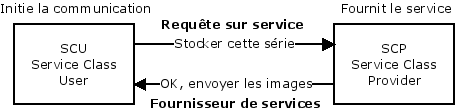
\includegraphics[width=.8\linewidth]{./figures/scu-scp.png}
	\end{center}
}

\frame
{
	\frametitle{Changement de r\^ole}
	Un \'equipement peut changer de r\^ole.
	
	Par exemple, une station d'interpr\'etation A peut \^etre :
	\begin{itemize}
		\item SCU dans un premier temps :
		\begin{enumerate}
			\item A sollicite un examen au PACS ;
			\item Le PACS accepte et envoie l'examen \`a A.
		\end{enumerate}
		\item puis SCP dans un second temps :
		\begin{enumerate}
		\setcounter{enumi}{2}
			\item B demande l'examen \`a A ;
			\item A transmet l'examen \`a B.
		\end{enumerate}
	\end{itemize}
	
%	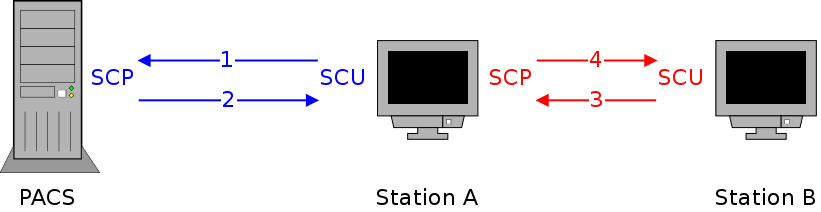
\includegraphics[width=\linewidth]{./figures/roles.png}
	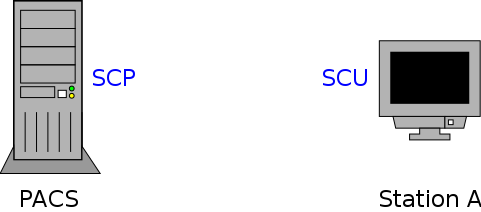
\includegraphics[width=.6\linewidth]{./figures/roles-scu.png}
	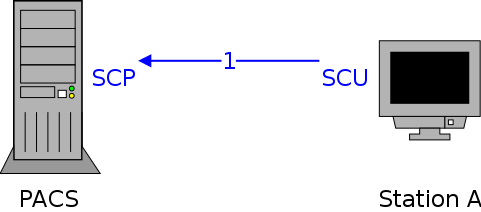
\includegraphics[width=.6\linewidth]{./figures/roles-1.png}
	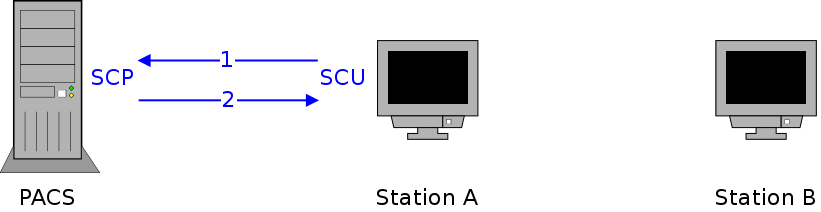
\includegraphics[width=.6\linewidth]{./figures/roles-2.png}
	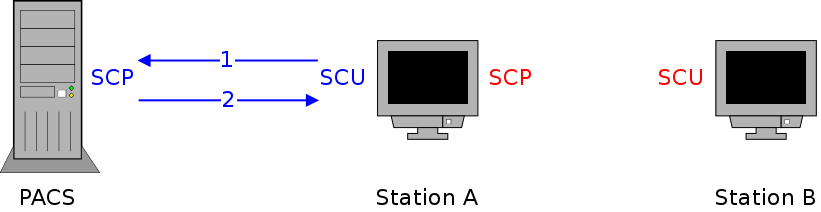
\includegraphics[width=\linewidth]{./figures/roles-scp.png}
	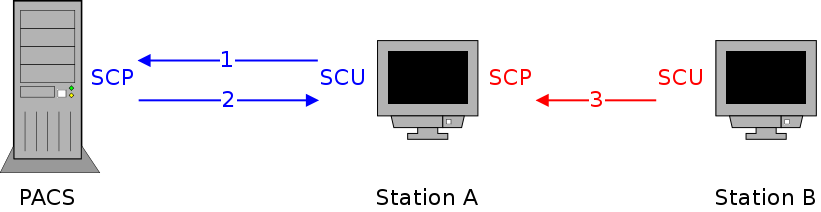
\includegraphics[width=\linewidth]{./figures/roles-3.png}
	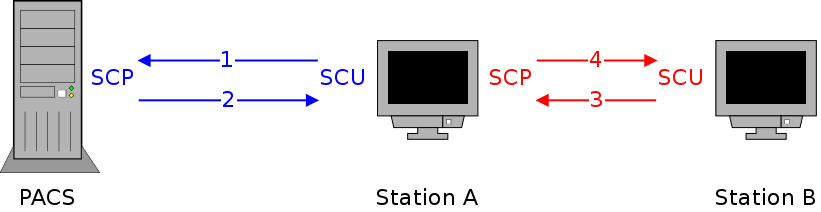
\includegraphics[width=\linewidth]{./figures/roles-4.png}
}

